%文責:黒崎・小出
%***各項目の執筆担当者名は最後に消してください

\subsection{初期運用}
%画像のファイル名は「3-4-Ini-1.jpg」「3-4-Ini-2.jpg」...
%ラベル名は「fig3-4-Ini-1」「fig3-4-Ini-2」...

\subsubsection{初期運用概要(黒崎)}
初期運用では,放出直後に地上との通信を行うため,アンテナの展開を試みるフェーズである.アンテナを収納する際に巻かれたテグスを溶断することでアンテナの展開を行う.以下に初期運用の簡単な流れを示す.

\begin{itemize}
	\item[1] OBCまたはCOBCが溶断する
	\item[2] 溶断が完了しアンテナが展開し,CW HKダウンリンクが開始する
	\item[3] CW HKダウンリンクが地上局で確認されたら,溶断停止コマンドを東工大地上局からアップリンクを行う
	\item[4] 衛星が溶断停止コマンドを受信したら,溶断を停止し,初期運用モードから定常運用モードに移行する
	\item[5] CW HKダウンリンクの溶断ステータスが溶断前から溶断済みに更新されていることを確認することで,衛星が定常運用モードに移行したことを地上局が認識する
\end{itemize}

\subsubsection{基本設計思想(黒崎・小出)}
\begin{itemize}
	\item \textbf{OBCがメインで溶断を行う.OBCが溶断に失敗している場合にCIBが溶断を行う.}本来であれば,SavingモードでOBCの電源が切られてしまうため,CIBがメインで溶断を行う方がシンプルな設計に出来た.しかし,CIBは初期運用以外の開発がかなり遅れていたため,初期運用のデバックに割ける時間が限られていること,またCIBに機能の集中を避けること,溶断の電源の供給の1つがOBCしか出来ないことなどを考慮し,OBCをメインにしたという背景がある.
	\item \textbf{溶断頻度は22.5分間隔.}これは地球1周を90分かけるOrigamiSat-1の軌道において,地球1周の間に4回溶断をトライする設計になっている.地球1周分を基準に考えているのは,日向,日陰条件で宇宙環境温度が異なり,溶断の成功確率に影響が出ることを考慮している.
	\item \textbf{1日の間で8回(地球2周分)溶断をトライした後は,溶断を行わず待機.}これはバッテリーを温存するためである.
\end{itemize}

\newpage
\subsubsection{開発の流れ(黒崎)}
開発の流れは以下の通りである.
\begin{itemize}
	\item[3-A] 不具合想定表作成
	\item[3-B] ソフトフローチャート作成
	\item[3-C] ソフト作成
	\item[3-D] デバック
	\item[3-E] フローチャートとソフトが対応しているか確認
	\item[3-F] OBC/CIB統合
	\item[3-G] 恒温槽試験で溶断時間の確認
	\item[3-H] FM最終確認
\end{itemize}

各工程の詳細を以下に示す.
\begin{itemize}
	\item[3-A] \textbf{不具合想定表作成}:不具合想定表は,「A)不具合原因表」と「B) 不具合対応表」からなる.
	
	A)不具合原因表は,電源系,通信系,その他の3種類に分けて作成した.実際に作成した表を表\ref{table3-4-Ini-0-a},表\ref{table3-4-Ini-0-b},表\ref{table3-4-Ini-0-c}に示す.表\ref{table3-4-Ini-0-a}に関しては,機器のトラブルによる再起動/電源オフだけでなく,モード切替による意図的な再起動/電源オフも想定している.
	
	B)不具合対応表は,各シークエンスにおいて,表\ref{table3-4-Ini-0-a},表\ref{table3-4-Ini-0-b},表\ref{table3-4-Ini-0-c}で想定された不具合が発生した場合の,①対処法(どのように冗長系を組むか),②デバックの際の検証方法を示している.OBC,RXPIC,TXPICそれぞれにおいて対応表を作成した.実際に作成した表を表\ref{table3-4-Ini-1},表\ref{table3-4-Ini-2},表\ref{table3-4-Ini-3}に示す.
	
	\newpage
	\begin{table}[H]
		\centering
		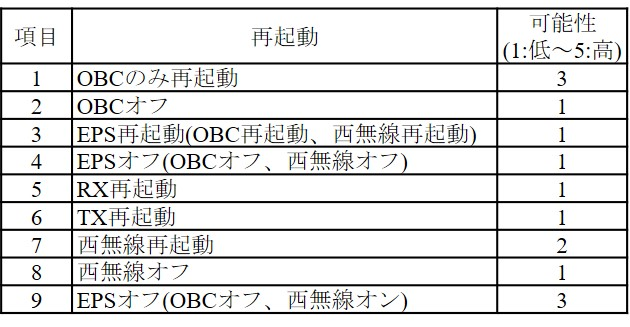
\includegraphics[scale=1]{03/fig/t3-4-Ini-0-a.jpg}
		\caption{不具合原因表(電源系)}
		\label{table3-4-Ini-0-a}
	\end{table}
	\begin{table}[H]
	\centering
	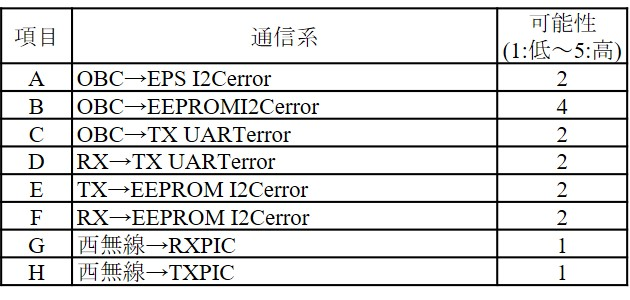
\includegraphics[scale=1]{03/fig/t3-4-Ini-0-b.jpg}
	\caption{不具合原因表(通信系)}
	\label{table3-4-Ini-0-b}
	\end{table}
	\begin{table}[H]
	\centering
	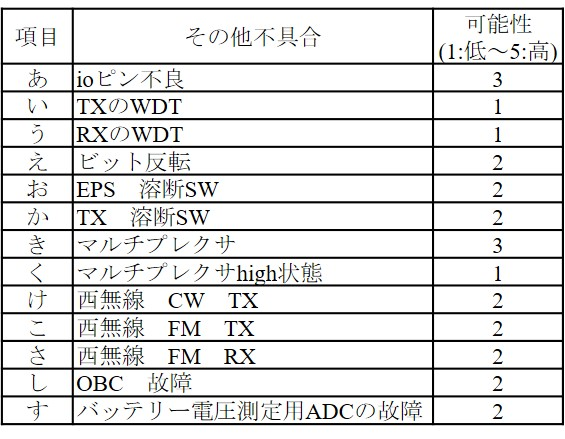
\includegraphics[scale=1]{03/fig/t3-4-Ini-0-c.jpg}
	\caption{不具合原因表(その他)}
	\label{table3-4-Ini-0-c}
	\end{table}
	\newpage
	
	\begin{table}[H]
		\centering
		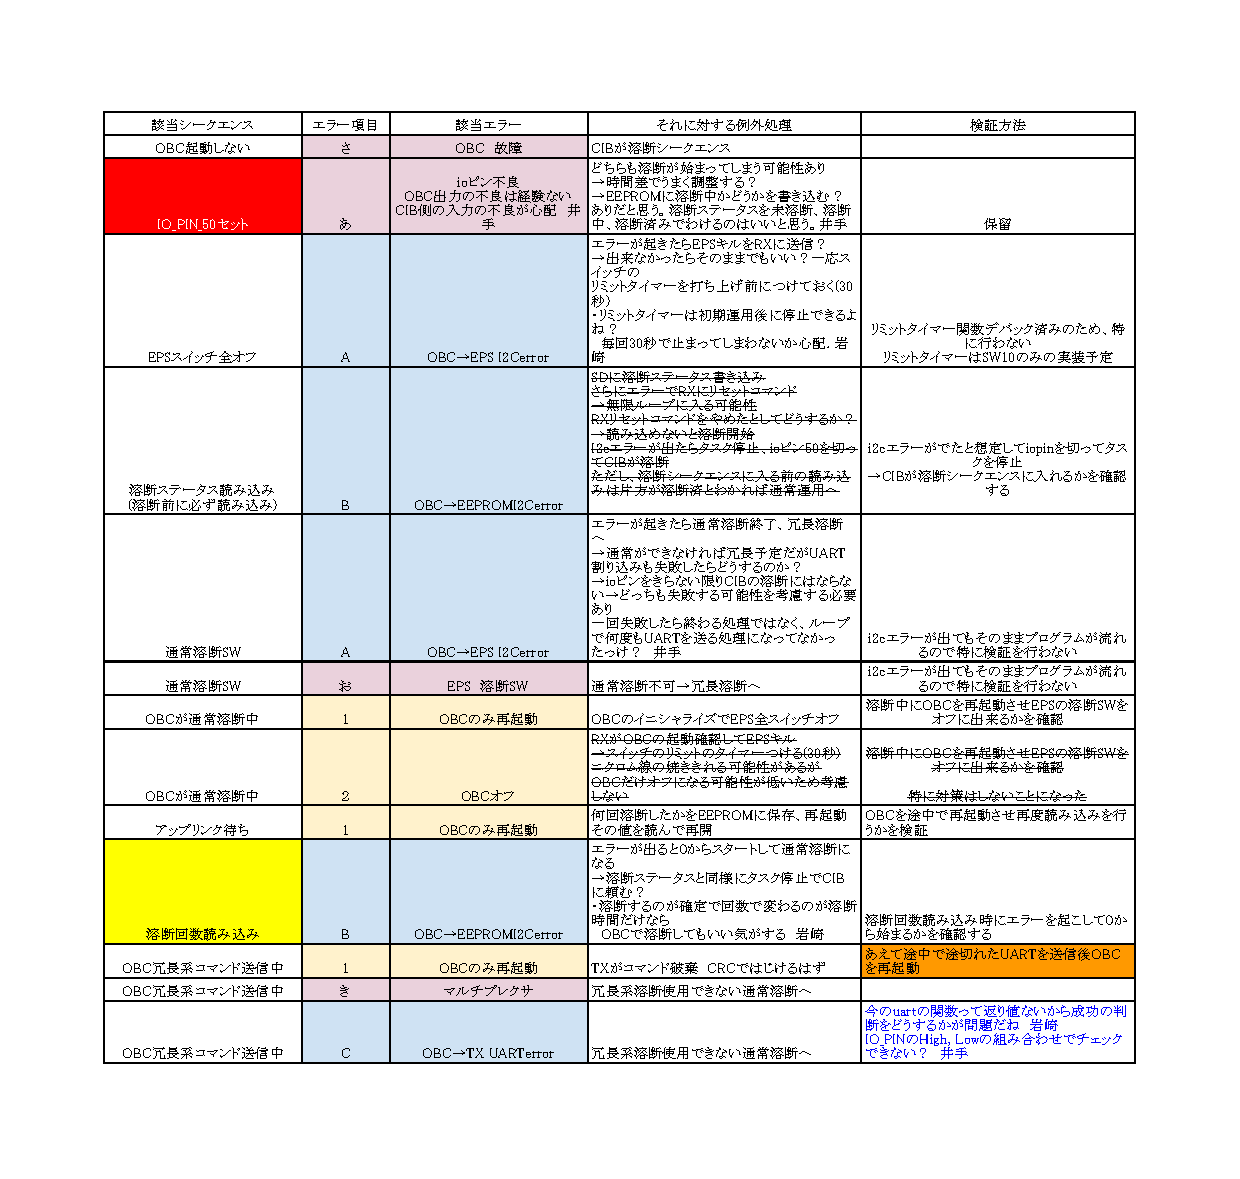
\includegraphics[scale=0.7]{03/fig/t3-4-Ini-1.pdf}
		\caption{不具合対応表(OBC)}
		\label{table3-4-Ini-1}
	\end{table}
	\begin{table}[H]
	\centering
	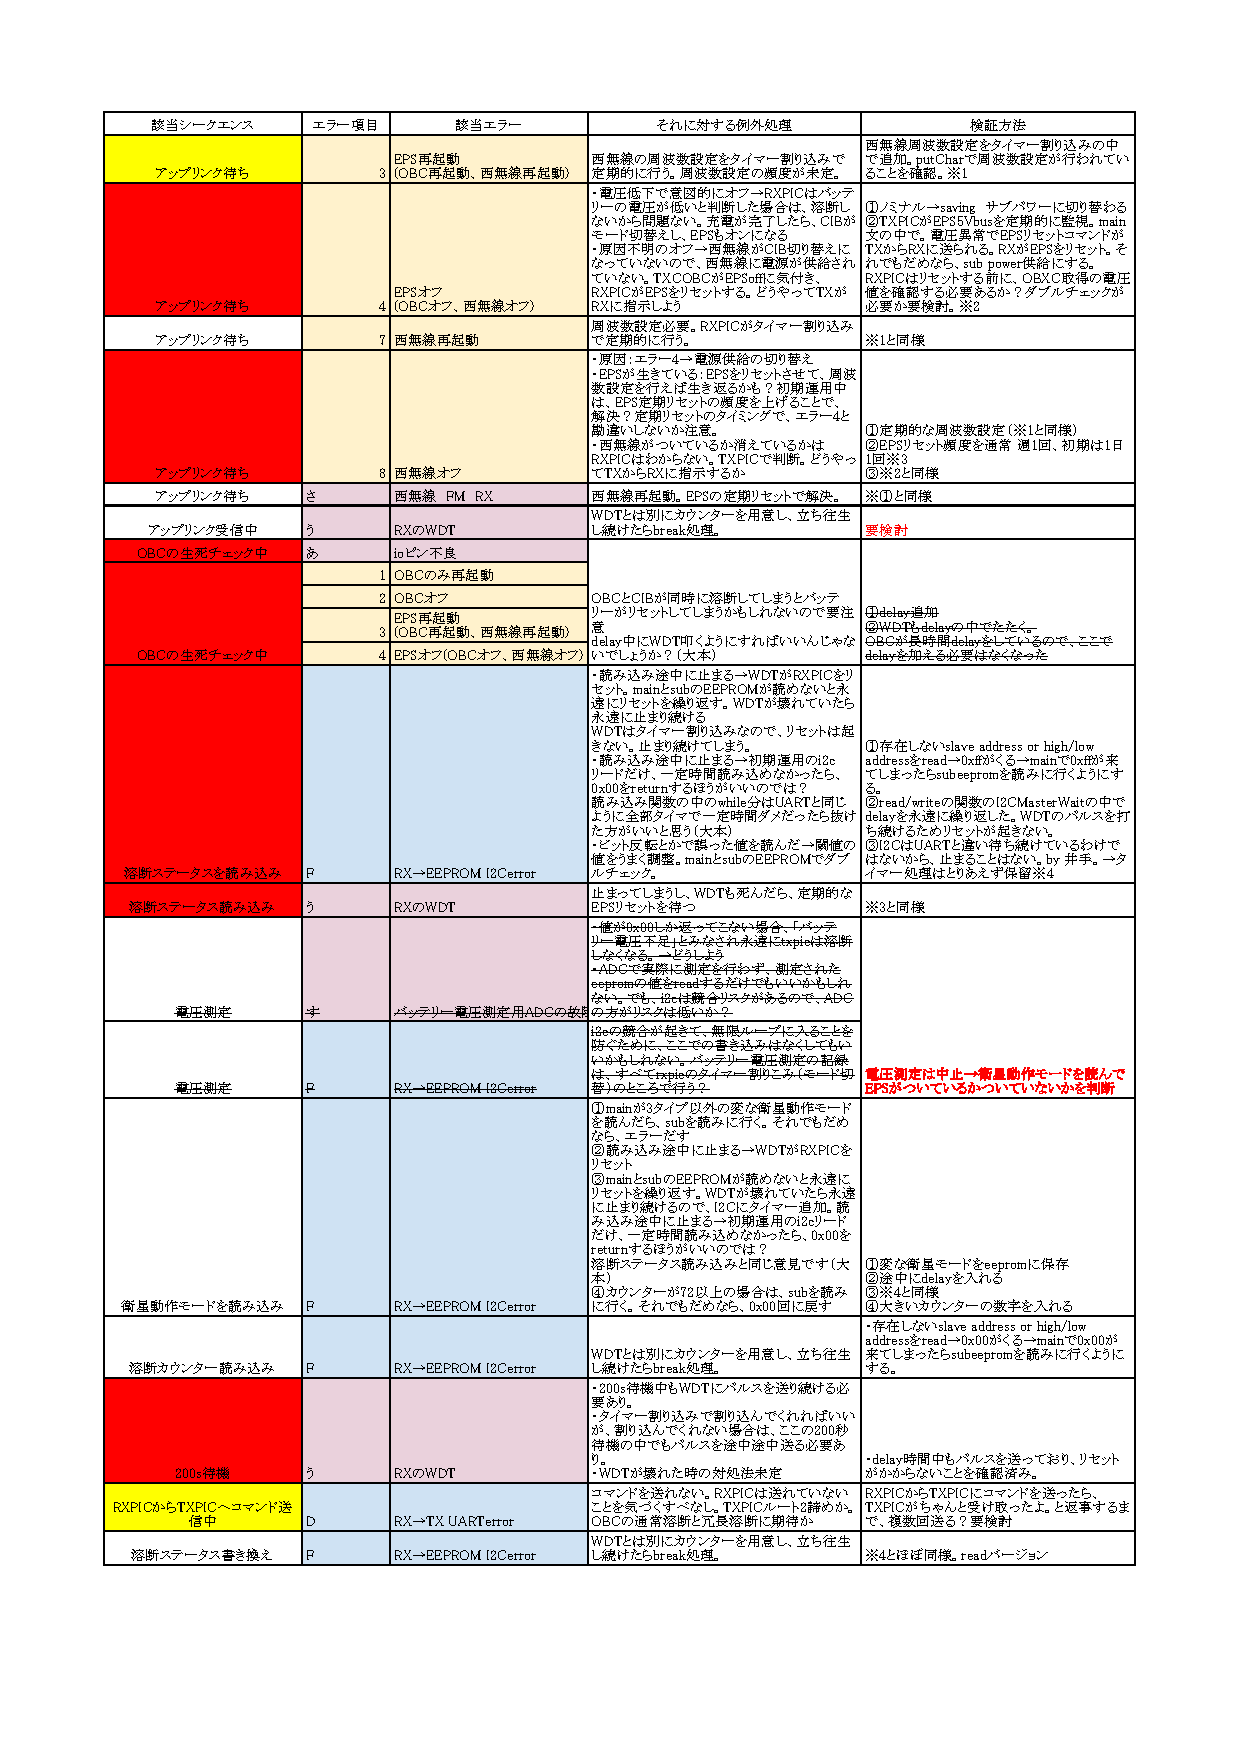
\includegraphics[scale=0.7]{03/fig/t3-4-Ini-2.pdf}
	\caption{不具合対応表(RXPIC)}
	\label{table3-4-Ini-2}
	\end{table}
	\begin{table}[H]
	\centering
	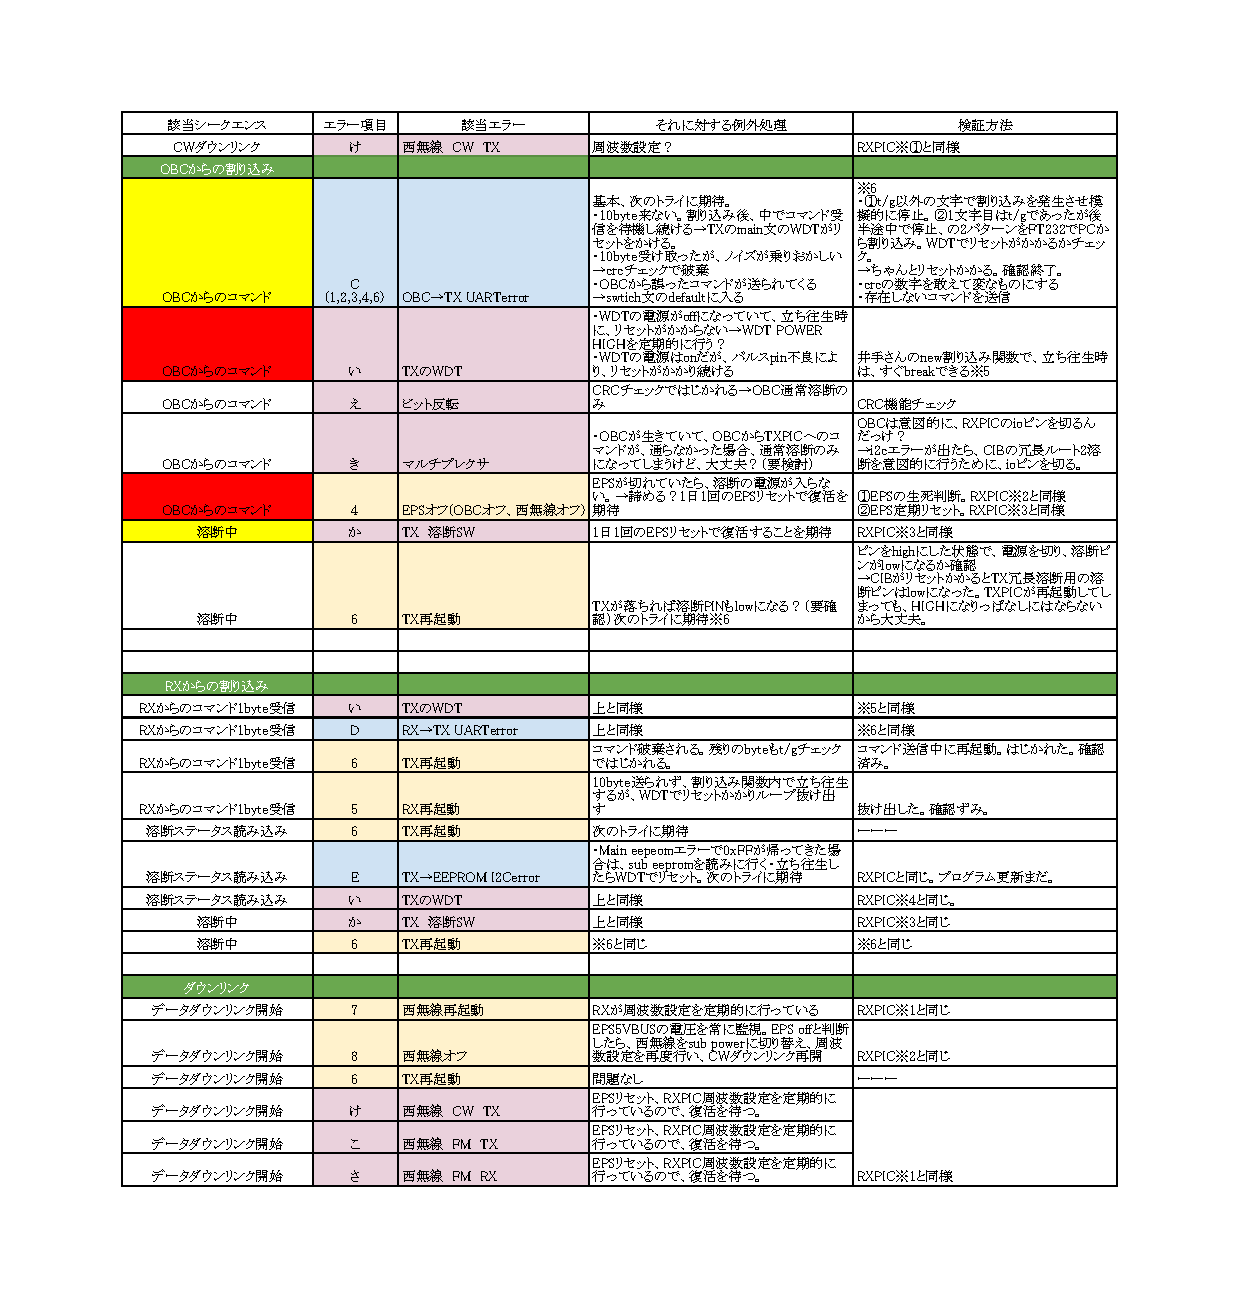
\includegraphics[scale=0.7]{03/fig/t3-4-Ini-3.pdf}
	\caption{不具合対応表(TXPIC)}
	\label{table3-4-Ini-3}
	\end{table}	

	%%%%%%%%%%%%%%%%%%%%%%%%%%
	\item[3-B] \textbf{ソフトフローチャート作成}:3-Aで作成した不具合想定表を元に,初期運用時のOBC,TXPIC,RXPICのフローチャートを作成した.作成したフローチャートは,他のコンポーネント担当者等とも検討した.
	
	\item[3-C] \textbf{ソフト作成}:3-Bで作成されたフローチャートを元に,ソフトを書いた.
	
	\item[3-D] \textbf{デバック}:3-Cと同時並行で書いたソフトをその都度デバックする.いつ,どの部分をデバックし,結果はどうであったかを必ず記録する.後に確認した際にどの部分までデバックしたか分からなくなってしまうため.
	
	\item[3-E] \textbf{フローチャートとソフトが対応しているか確認}
	\item[3-F] \textbf{OBC/CIB統合}.初期運用はOBCとCIBが連携して行うため,統合作業が必要である.冗長系を含むフローチャートの全てのルートにおいてバグが無いかを,単体では3-Dで確認済みだが,OBCとCIBのプログラムを同時に動かして確認した.
	\item[3-G] \textbf{恒温槽試験で溶断時間の確認}:恒温槽において,宇宙環境の想定最大温度50℃と想定最低温度-30℃を再現し,それぞれの温度環境下で溶断することができるか,溶断時間は適切であるか検証した.
	\item[3-H] \textbf{FM最終確認}:FM本体をJAXAに引き渡す直前,最終プログラム書き込み後,eeprom初期パラメータ書き込み前に,初期運用プログラムで溶断できるか確認を行った.FM本体を溶断することはできないので,ダミーの糸を溶断した.
	
\end{itemize}	

\subsubsection{OBC初期運用モードソフト詳細(小出)}
OBC正常時のフローチャートを以下に示す.
\begin{figure}[H]
	\centering
	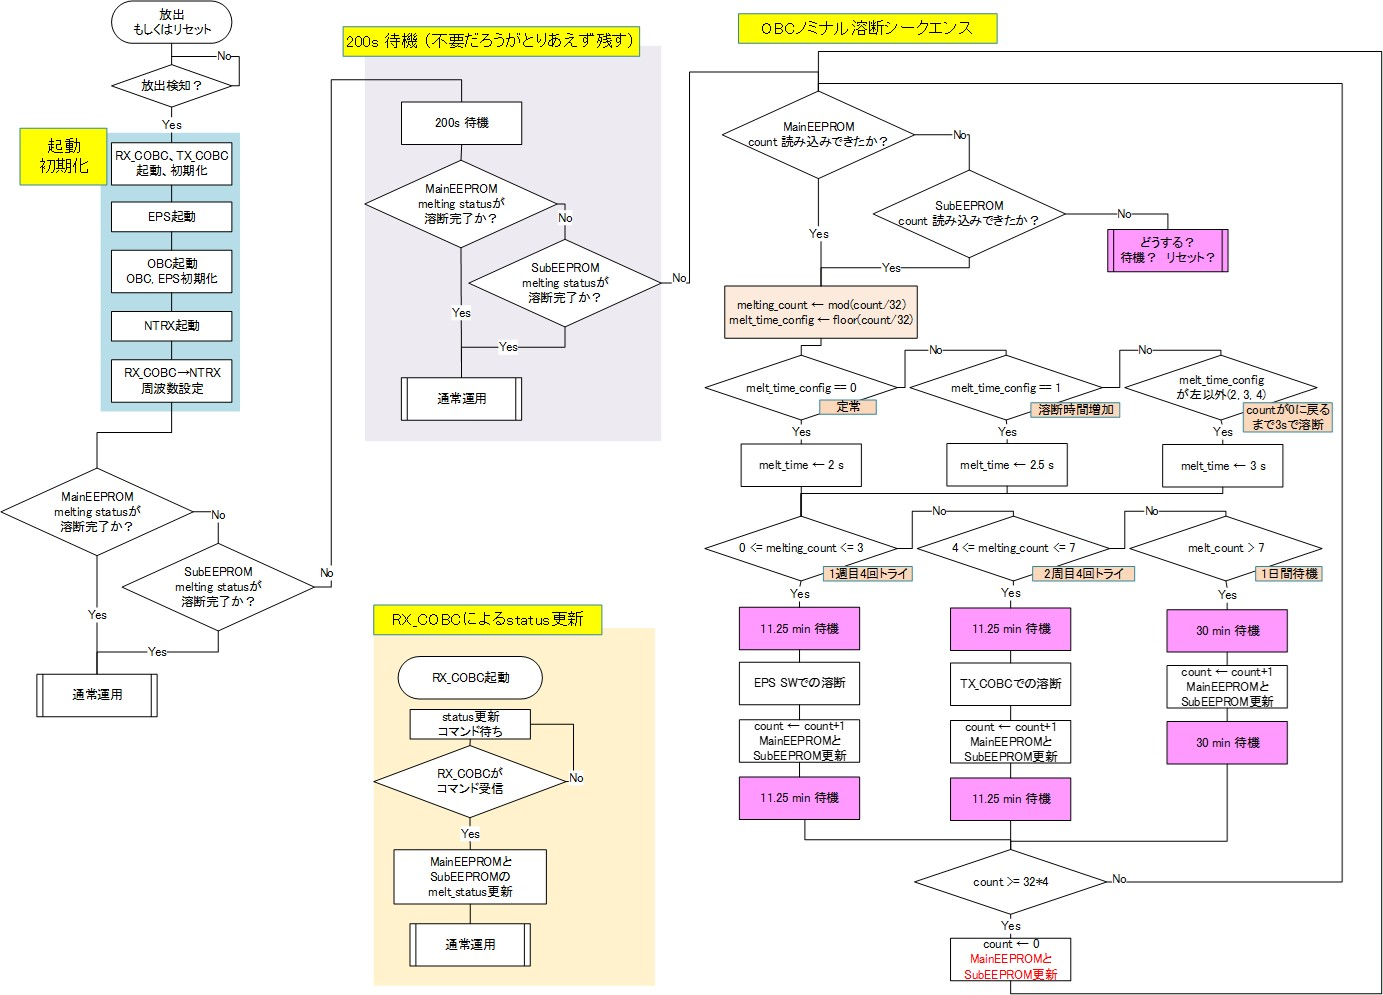
\includegraphics[scale=0.7]{03/fig/3-4-Ini-1.pdf}
	\caption{OBC正常時のフローチャート}
	\label{fig3-4-Ini-1}
\end{figure}	
\begin{itemize}
	\item OBCはRTOSを使い複数のタスクを持っているが起動時に動くのは初期運用のタスクのみ
	この時必ずCIBにOBCが起動しているかの確認を行うIOピンをhighにする
	\item EEPROMに書き込まれた溶断ステータスの計算式については1byteを1bitずつ加算その値が4以上だと溶断判断(CIB共通事項なのでどこに書くべきなのか要検討)
	\item countで溶断回数又は待機を判断OBCの電源を落ちることを考慮した
	\item OBCはEPSのWDTを管理しているので,初期運用時では初期運用のタスク内のループでたたきに行く構造(通常はOBCのコマンド確認で行っている詳細はOBCの章)
\end{itemize}
\subsubsection{CIB初期運用モードソフト詳細(黒崎)}
フローチャート的なものとセットで

\subsubsection{初期運用 運用結果(黒崎)}
%以下のアクションの日付を書き足したいな...
アマチュア無線家からのCW HKデータ受信報告を受け,東工大地上局にて溶断停止コマンドをアップリンク.CW HKデータで溶断ステータスが溶断前から溶断済みに書き換わっていることを確認した.

\subsubsection{コメントや次回の改善点}
\hspace{2ex}
\textbf{OBC / CIB共通(黒崎・小出)}
\begin{itemize}
	\item 溶断済みフラグをCW HKデータのフリースペースの1byteに入れたのは神采配だったと思う.OrigamiSat-1の場合,アップリンクでEEPROMの指定アドレスを読んでダウンリンクする機能が使えなくなってしまっていたため,CW HKデータ以外に溶断済みを確認する術が無かった.
	\item OBCとCIBが同時に溶断を行ってしまった場合,バッテリーがどの程度減少するかの検証をできていなかった.
	\item OBCとCIBのどちらが,何回目の溶断で溶断を成功し,ダウンリンクを開始したかを分かるようにした方がいいのかもしれない.
	\item 「(3)開発の流れ」3-FにおけるOBC/CIBの統合は,初期運用のプログラムしか動かしていなかったので,モード切替やダウンリンクなども動かし,本番の運用を想定したデバックが必要であった.
\end{itemize}

\hspace{2ex}
\textbf{OBC(小出)}
\begin{itemize}
	\item aaaaaaaa
\end{itemize}

\hspace{2ex}
\textbf{CIB(黒崎)}
\begin{itemize}
	\item FMに書き込んだプログラムでは,溶断ステータスは毎回,eepromを読み込んで判断としていたが,一度,溶断停止コマンドがアップリンクされて溶断ステータスが書き換わったら,PIC内のグローバル変数も書き換わるようなプログラムの方が良かったかもしれない.
	
	というのも,RXPICがeepromの読み込みができず,溶断ステータスを判断できない場合は全て「未溶断」判定にしていた.実際,OrigamiSat-1はeepromを読み込めないとい事象が起きてしまい,RXPICは毎回,初期運用モードに入り,200秒待機や溶断などをしてしまっていたと思われるため.
\end{itemize}